% --- Template for thesis / report with tktltiki2 class ---
% 
% last updated 2013/02/15 for tkltiki2 v1.02

\documentclass[finnish]{tktltiki2}

% tktltiki2 automatically loads babel, so you can simply
% give the language parameter (e.g. finnish, swedish, english, british) as
% a parameter for the class: \documentclass[finnish]{tktltiki2}.
% The information on title and abstract is generated automatically depending on
% the language, see below if you need to change any of these manually.
% 
% Class options:
% - grading                 -- Print labels for grading information on the front page.
% - disablelastpagecounter  -- Disables the automatic generation of page number information
%                              in the abstract. See also \numberofpagesinformation{} command below.
%
% The class also respects the following options of article class:
%   10pt, 11pt, 12pt, final, draft, oneside, twoside,
%   openright, openany, onecolumn, twocolumn, leqno, fleqn
%
% The default font size is 11pt. The paper size used is A4, other sizes are not supported.
%
% rubber: module pdftex

% --- General packages ---

\usepackage[utf8]{inputenc}
\usepackage[T1]{fontenc}
\usepackage{lmodern}
\usepackage{microtype}
\usepackage{amsfonts,amsmath,amssymb,amsthm,booktabs,color,enumitem,graphicx}
\usepackage[pdftex,hidelinks]{hyperref}
\usepackage{verbatim}
\usepackage{ragged2e}

% Use section based figure numbering.
\usepackage{chngcntr}
\counterwithin{figure}{section}

\usepackage{listings}
\usepackage{color}
\definecolor{lightgray}{rgb}{.92,.92,.92}
\definecolor{darkgray}{rgb}{.4,.4,.4}
\definecolor{purple}{rgb}{0.65, 0.12, 0.82}
\lstdefinelanguage{JavaScript}{
  keywords={break, case, catch, continue, debugger, default, delete, do, else, false, finally, for, function, if, in, instanceof, new, null, return, switch, this, throw, true, try, typeof, var, void, while, with},
  morecomment=[l]{//},
  morecomment=[s]{/*}{*/},
  morestring=[b]',
  morestring=[b]",
  ndkeywords={class, export, boolean, throw, implements, import, this},
  keywordstyle=\color{blue}\bfseries,
  ndkeywordstyle=\color{darkgray}\bfseries,
  identifierstyle=\color{black},
  commentstyle=\color{purple}\ttfamily,
  stringstyle=\color{red}\ttfamily,
  sensitive=true
}

\lstset{
   language=JavaScript,
   backgroundcolor=\color{lightgray},
   extendedchars=true,
   literate={ä}{{\"a}}1 {ö}{{\"o}}1,
   basicstyle=\footnotesize\ttfamily,
   showstringspaces=false,
   showspaces=false,
   numbers=left,
   numberstyle=\footnotesize,
   numbersep=9pt,
   tabsize=2,
   breaklines=true,
   showtabs=false,
   captionpos=b
}

\graphicspath{{images/}}

% Automatically set the PDF metadata fields
\makeatletter
\AtBeginDocument{\hypersetup{pdftitle = {\@title}, pdfauthor = {\@author}}}
\makeatother

% babelbib for non-english bibliography using bibtex
\usepackage[fixlanguage]{babelbib}
\selectbiblanguage{finnish}

% Hack with negative space to fix space before full stop.
\declarebtxcommands{finnish}{%
\def\btxurldatecomment#1{, vierailtu #1\!\!}%
}

% Remove [brackets] around keys.
\makeatletter
\renewcommand\@biblabel[1]{\hfill #1.}
\makeatother

% Try not to break small words. (että, jotta, etc.) (range: 0 - 10 000)
\pretolerance=1000

% add bibliography to the table of contents
\usepackage[nottoc]{tocbibind}
% tocbibind renames the bibliography, use the following to change it back
\settocbibname{Lähteet}

% --- Theorem environment definitions ---

\newtheorem{lau}{Lause}
\newtheorem{lem}[lau]{Lemma}
\newtheorem{kor}[lau]{Korollaari}

\theoremstyle{definition}
\newtheorem{maar}[lau]{Määritelmä}
\newtheorem{ong}{Ongelma}
\newtheorem{alg}[lau]{Algoritmi}
\newtheorem{esim}[lau]{Esimerkki}

\theoremstyle{remark}
\newtheorem*{huom}{Huomautus}

% --- tktltiki2 options ---

\title{JavaScript ja virtuaalikoneet}
\author{Ville Lahdenvuo}
\date{\today}
\level{Kandidaatintutkielma}
\abstract{
  \renewcommand{\baselinestretch}{1.5}
  \selectfont
  JavaScript-virtuaalikoneet ovat perinteisesti toimineet tulkkaamalla lähdekoodista muodostettua abstraktia syntaksipuuta tai tavukoodia. Virtuaalikoneissa on otettu käyttöön monenlaisia JIT-kääntäjiä, mutta tulkkia käytetään yhä varsinkin suorituksen alussa sen keveyden ja nopeuden takia. JavaScriptin dynaamisuudesta johtuen virtuaalikoneiden kehittäjät ovat joutuneet toteuttamaan monimutkaisia menetelmiä tehokkaan konekoodin tuottamiseksi JavaScript-ohjelmista.

Monet optimoinnit käyttävät hyväksi oletusta, että sovellukset käyttäytyvät melko staattisesti, kielen dynaamisuudesta huolimatta. Tämän oletuksen nojalla on pystytty hyödyntämään optimointimenetelmiä, joita tyypillisesti käytetään staattisesti tyypitettyjen kielten kanssa.

Oletus staattisesta käytöksestä on havaittu ongelmalliseksi. Vaikka yleisesti käytössä olevat suorituskykytestit käyttäytyvät varsin staattisesti, todelliset sovellukset hyödyntävät kielen dynaamisuutta enemmän, mikä heikentää optimointimenetelmien toimivuutta.
}

% The following can be used to specify keywords and classification of the paper:

\keywords{JavaScript, virtuaalikone, suorituskyky}

% Classification according to ACM Computing Classification System (http://www.acm.org/about/class/)
%
% Software and its engineering
%   Software organization and properties
%     Contextual software domains
%       Software infrastructure
%         Virtual machines
%   Software notations and tools
%     General programming languages
%       Language types
%         Very high level languages

\classification{
  \textbf{Software and its engineering $\rightarrow$ Virtual machines} \\
  Software and its engineering $\rightarrow$ Very high level languages
}

% If the automatic page number counting is not working as desired in your case,
% uncomment the following to manually set the number of pages displayed in the abstract page:
%
% \numberofpagesinformation{16 sivua + 10 sivua liitteissä}

\begin{document}

% --- Front matter ---

\frontmatter      % roman page numbering for front matter

\maketitle        % title page
\makeabstract     % abstract page

\tableofcontents  % table of contents

% --- Main matter ---

\mainmatter       % clear page, start arabic page numbering

% Set bigger space between lines.
\renewcommand{\baselinestretch}{1.5}
\selectfont

%\noindent
JavaScript on ohjelmointikieli, joka suunniteltiin ensisijaisesti verkkosivujen tekijöille, joilla ei välttämättä ole paljon ohjelmointikokemusta. Sen idea oli täydentää Java-ohjelmointikieltä ja HTML-merkkauskieltä. Se mahdollistaa monimutkaisten Internet-selaimissa suoritettavien sovellusten kirjoittamisen ilman selainlaajennuksia~\cite{paolini1994netscape}.

Selainten suosio sovellusalustana on kasvanut ja samalla JavaScriptin käyttö on lisääntynyt räjähdysmäisesti. Se ei ole yllättävää, sillä kaikissa kuluttajatietokoneissa on jokin selain. Lisäksi sovellusten jakaminen on helppoa, koska siihen riittää pelkkä URL-osoite.

Selaimet ovat kehittyneet ja niiden käyttämiä teknologioita on standardoitu. Tämä on auttanut tekemään JavaScriptistä varteenotettavan vaihtoehdon moderniin sovelluskehitykseen. JavaScriptin käyttö ei kuitenkaan rajoitu vain selaimiin, vaan sitä käytetään myös palvelinsovelluksissa sekä muissa ilman selainta toimivissa sovelluksissa, kuten esimerkiksi Atom-tekstieditorissa~\cite{atom}.

JavaScript on dynaaminen oliopohjainen kieli, mutta se tukee myös imperatiivista ja funktionaalista ohjelmointityyliä. JavaScript siis tarjoaa monta tapaa toteuttaa samoja asioita~\cite[Osio 4.2.1.]{es6}. Muuttujat JavaScriptissä ovat dynaamisesti tyypitettyjä ja tämä helpottaa ohjelmointia tekemällä muuttujien käytöstä vapaampaa. Tästä dynaamisuudesta seuraa kuitenkin myös ongelmia, sillä virtuaalikoneiden on vaikea ennustaa dynaamisia muutoksia ja tehdä järkeviä optimointeja, joilla suorituskykyä saisi parannettua~\cite{Ahn2014}.

Modernit JavaScript-virtuaalikoneet ovat kehittyneet paljon viime vuosina ja niihin on toteutettu monimutkaisia ja kekseliäitä menetelmiä suorituskyvyn parantamiseksi. Esimerkkejä tälläisistä ovat muun muassa piiloluokat (hidden classes) ja erilaiset ajonaikaiset optimoivat kääntäjät.

Suuri osa virtuaalikoneiden parannuksista perustuvat oletukseen, että vaikka kieli itsessään on dynaaminen, ohjelmat kuitenkin käyttäytyvät yleensä melko staattisesti. Keräämällä tyyppitietoa suorituksen aikana, virtuaalikoneet pystyvät esimerkiksi luomaan optimoitua konekoodia osalle lähdekoodista. Tämä edellyttää tietenkin, että JavaScript-ohjelmoija tietää miten asiat kannattaa toteuttaa.

Kieltä kuitenkin kehitetään jatkuvasti ja siihen ollaan tuomassa muun muassa luokka- ja moduulijärjestelmät~\cite[Osiot~14.5.~ja~15.2.]{es6}, jotka pyrkivät yhtenäistämään toteutustapoja ja mahdollistavat tällä tavoin paremman ennustettavuuden ja suorituskyvyn.

On selvää, että JavaScriptin standardoiminen, sen käytön lisääntyminen ja selainvalmistajien keskinäinen kilpailu suorituskyvystä on parantanut kielen asemaa ja mainetta. JavaScriptin rooli on muuttunut skriptikielestä yleiskäyttöiseksi ohjelmointikieleksi~\cite[Osio~4.]{es6}. Kielen tulevaisuus näyttää lupaavalta. Siihen on tulossa paljon ohjelmointia helpottavia ominaisuuksia ja tapoja välttää yleisiä sudenkuoppia, joihin varsinkin aloittelevat ohjelmoijat usein törmäävät.
\section{Johdanto}

JavaScript on ohjelmointikieli, joka suunniteltiin ensisijaisesti verkkosivujen tekijöille. Sen tavoite oli täydentää Java-ohjelmointikieltä ja HTML-merkkauskieltä. JavaScript mahdollistaa monimutkaisten Internet-selaimissa suoritettavien sovellusten kirjoittamisen ilman selainlaajennuksia~\cite{paolini1994netscape}.

Selainten suosio sovellusalustana on kasvanut ja samalla JavaScriptin käyttö on lisääntynyt paljon. Kasvua siivittää se, että kaikissa kuluttajatietokoneissa on jokin selain ja sovellusten käyttämiseen riittää verkkosivuilla vieraileminen. Käyttäjän ei tarvitse asentaa mitään ennen sovelluksen käyttöä.

Selaimet ovat kehittyneet ja niiden käyttämiä teknologioita on standardisoitu. Näistä niin sanotuista Web-teknologioista, joihin JavaScript lasketaan, on tullut varteenotettava vaihtoehto moderniin sovelluskehitykseen. Web-teknologioiden käyttö ei kuitenkaan rajoitu vain selaimiin. Niillä on toteutettu esimerkiksi palvelinsovelluksia sekä kokonaan ilman selainta toimivia sovelluksia, kuten Atom-tekstieditori~\cite{atom}.

JavaScript on dynaaminen oliopohjainen kieli, mutta se tukee myös imperatiivista ja funktionaalista ohjelmointityyliä. JavaScript tarjoaa siis monia tapoja toteuttaa sama asia~\cite[4.2.1.]{es6}. Muuttujat JavaScriptissä ovat dynaamisesti tyypitettyjä ja tämä helpottaa ohjelmakoodin kirjoittamista. Dynaamisuudesta seuraa kuitenkin myös ongelmia, sillä virtuaalikoneiden on vaikea ennustaa dynaamisia muutoksia ja tehdä järkeviä optimointeja, joilla suorituskykyä voitaisiin parantaa~\cite[s.~497]{Ahn2014}.

Modernit JavaScript-virtuaalikoneet ovat kehittyneet paljon viime vuosina. Niihin on toteutettu monimutkaisia ja kekseliäitä menetelmiä suorituskyvyn parantamiseksi. Suuri osa virtuaalikoneiden optimoinneista perustuu oletukseen, että dynaamisuudesta huolimatta ohjelmat käyttäytyvät suorituksen aikana yleensä melko staattisesti. Keräämällä tyyppitietoa suorituksen aikana, virtuaalikoneet pystyvät esimerkiksi luomaan optimoitua konekoodia osalle lähdekoodista. Optimoitavuus edellyttää, että ohjelmoija tietää miten asiat kannattaa toteuttaa. Jos hyödyntää dynaamisuutta liikaa, voi helposti tehdä koodia, jota virtuaalikone ei pysty optimoimaan.

%Esimerkkejä tälläisistä ovat muun muassa \textit{piiloluokat} (hidden classes)~\cite{v8design} ja erilaiset suorituksenaikaiset optimoivat kääntäjät. Piiloluokat ovat staattisia luokkia, joita virtuaalikone käyttää objektien kuvaamiseen. Jos objektia muutetaan, esimerkiksi lisäämällä uusi kenttä, luodaan sille uusi piiloluokka. Piiloluokkien hyödyt tulevat esiin, jos ohjelmassa on paljon samanlaisia objekteja, jotka voivat käyttää samaa piiloluokkaa.

JavaScriptiä kuitenkin kehitetään jatkuvasti ja siihen on tuotu muun muassa luokka- ja moduulijärjestelmät~\cite[14.5.~ja~15.2.]{es6}. Nämä auttavat yhtenäistämään erilaisia toteutustapoja ja mahdollistavat tällä tavoin aikaisempaa paremmin ennustettavan käytöksen. Kun käytetään luokkasyntaksia, tulee käytettyä yhtenäistä tapaa muodostaa objekteja. Ennustettavuudesta seuraa parempi optimoitavuus ja suorituskyky~\cite[s.~497]{Ahn2014}.

JavaScriptin standardisoiminen, sen käytön lisääntyminen ja selainvalmistajien keskinäinen kilpailu suorituskyvystä on parantanut kielen asemaa ja mainetta. JavaScriptin rooli on muuttunut skriptikielestä yleiskäyttöiseksi ohjelmointikieleksi~\cite[4.]{es6}. Kielen tulevaisuus näyttää lupaavalta. Siihen on tullut paljon ohjelmointia helpottavia ominaisuuksia ja tapoja välttää yleisiä sudenkuoppia, joihin varsinkin aloittelevat ohjelmoijat usein törmäävät.
\section{Virtuaalikoneiden toiminta}

Virtuaalikone on ohjelma, joka tarjoaa todellisen tai hypoteettisen laitteen toiminnallisuuksia muille ohjelmille hyödyntäen sitä suorittavan \textit{isäntäjärjestelmän} abstraktioita. Virtuaalikone voi esimerkiksi virtualisoida optista asemaa käyttämällä isännän tiedostojärjestelmää hyväksi, jolloin virtuaalikoneessa suoritettava ohjelma luulee lukevansa optista levyä, kun todellisuudessa tieto tulee kiintolevyltä. Virtuaalikoneita on kahdenlaisia, \textit{järjestelmä-} ja \textit{prosessivirtuaalikoneita}~\cite[s.~33]{vms}. Järjestelmävirtuaalikone tarjoaa kokonaisen käyttöjärjestelmän palvelut toisin kuin prosessivirtuaalikone, joka tarjoaa vaan yhden prosessin suorittamista varten tarvittavat palvelut.

\subsection{Virtuaalikoneen anatomia}

Tässä tutkielmassa virtuaalikoneella tarkoitetaan korkean tason ohjelmointikielellä toteutetun ohjelman suorittavaa virtuaalikonetta. Tällaiset virtuaalikoneet ovat prosessivirtuaalikoneita. Ohjelma riittää kääntää virtuaalikoneelle, jolloin se toimii kaikilla alustoilla, joille kyseinen virtuaalikone on toteutettu.

Virtuaalikonemalli parantaa myös tietoturvaa. Virtuaalikoneessa suoritettava ohjelma pääsee käsiksi vain virtuaalikoneen tarjoamiin palveluihin, jolloin ohjelmat on helpompi eristää käyttöjärjestelmästä ja laitteistosta~\cite[s.~36]{vms}. Pahan tahtoisen ohjelman on siis löydettävä haavoittuvuus sekä virtuaalikoneesta että sen isännästä.

Ensimmäisen JavaScript-virtuaalikoneen nimi on SpiderMonkey~\cite{spidermonkey}. Se toteutettiin Netscape-selainta varten vuonna 1995 ja nykyään sitä ylläpitää Mozilla ja sitä käytetään muun muassa Mozillan Firefox-selaimessa. Nykyinen SpiderMonkey koostuu kolmesta fundamentaalisesta komponentista: \textit{kääntäjä}, \textit{tulkki} ja \textit{roskienkerääjä}~\cite{spidermonkeydesign}.

Kääntäjä huolehtii koodin \textit{jäsentämisestä} (parsing) ja kääntämisestä \textit{tavukoodiksi}. Virtuaalikoneen tavukoodi on verrattavissa todellisen koneen konekoodiin. Sitä on helpompi käsitellä ohjelmallisesti kuin tekstimuotoista ohjelmakoodia, sillä se on yksinkertaisempaa syntaksiltaan, joskin runsassanaisempaa.

Tulkin tehtävä on suorittaa tavukoodia. Tulkki siis lukee tavukoodia ja tekee tarvittavat toiminnot, jotka riippuvat alustasta. Tulkista on siis oltava oma versionsa jokaista tuettua alustaa varten. Todellisuudessa tulkkia käytetään vain suorituksen alkuvaiheessa keräämään tyyppitietoa. Usein kutsutut, niin sanotut ``kuumat'' funktiot, pyritään kääntämään optimoiduksi konekoodiksi \textit{suorituksenaikaisella kääntäjällä} eli \textit{JIT-kääntäjällä} (Just-In-Time compiler)~[lähde?].

Roskienkerääjän tehtävä on yksinkertaisesti poistaa muistista muuttujat ja oliot, joihin ohjelmassa ei enää viitata. Roskienkerääjän ansiosta ohjelmoijan ei tarvitse vapauttaa muistia itse, vaan järjestelmä hoitaa muistinhallinnan automaattisesti. Automaattinen muistinhallinta vähentää virheiden määrää, kuten muistivuotoja, mutta ei poista kaikkia ongelmia~[lähde?].

\subsection{Esimerkki: V8}

Vuonna 2008 Google julkaisi uuden selaimen, Google Chromen, jonka oli tarkoitus parantaa verkkosovellusten käyttökokemusta~\cite{chromepress}. Googlen kiinnostus käyttökokemuksen parantamisesta on ymmärrettävää, sillä yhtiöllä on paljon verkkopalveluita, jotka hyötyvät hyvästä suorituskyvystä. Näistä syistä Google päätyi toteuttamaan oman JavaScript-virtuaalikoneen V8:n.

Mielenkiintoisen V8:sta tekee se, että siinä ei ole lainkaan tulkkia. Sen sijaan V8 kääntää JavaScript koodin suoraan konekoodiksi ennen suorittamista. SpiderMonkeyn tapaan se kerää tyyppitietoa suorituksen aikana ja käyttää optimoivaa JIT-kääntäjää suorituskyvyn parantamiseksi~\cite{v8compilers}.

%V8:ssa on luonnollisesti myös roskienkerääjä, sillä kielen standardiin kuuluu automaattinen muistinhallinta. Muistinhallinnasta kerrotaan lisää sen suorituskykyä käsittelevässä kappaleessa.

\subsection{Esimerkki: JavaScriptCore}

JavaScriptCore on WebKit-nimisen Web-teknologioita toteuttavan ohjelmistokomponentin JavaScript-virtuaalikone. Apple käyttää WebKitiä ja \mbox{JavaScriptCorea} Safari-selaimessaan.

JavaScriptCore koostuu tulkista, yksinkertaisesta JIT-kääntäjästä sekä Googlen V8:n innoittamana optimoivasta JIT-kääntäjästä, jota he kutsuvat nimellä DFG-JIT. DFG tulee sanoista \textit{Data Flow Graph}, joka kuvaa ohjelman suorituksenaikaisen tyyppitiedon tallentavaa tietorakennetta. Eli kuten aikaisempien esimerkkien kohdalla, virtuaalikone ensin kerää tyyppitietoa ja sitten generoi optimoitua konekoodia~\cite{javascriptcore}.

\subsection{Esimerkki: Chakra}

Tekstiä tähän...

\subsection{JavaScriptin tuomat haasteet}

Kuten aikaisemmista esimerkeistä käy ilmi, virtuaalikoneet eivät voi suoraan generoida optimoitua konekoodia JavaScript-ohjelmista, sillä ei ole tietoa muuttujien tyypeistä. Prosessorin kannalta on hyvin tärkeää tietää tehdäänkö jokin operaatio kokonaisluvuille, liukuluvuille vai kenties merkkijonoille.

Automaattinen roskienkeruu on todella kätevä toiminnallisuus ohjelmoijan kannalta, mutta sen toteuttaminen hyvin on haastavaa. Ohjelman on pysähdyttävä ja käytävä läpi muistin sisältöä ja vapauttaa muistialueita, jotka eivät ole enää käytössä. Selaimen tapauksessa tämä voi aiheuttaa verkkosovelluksen hidastumista ja huonontaa käyttökokemusta, varsinkin jos kyseessä on interaktiivinen toiminto tai animaatio.
\section{Optimointimenetelmät}

Konekoodiksi kääntäminen tuo ongelmaksi hitaan käännösvaiheen. Tämän takia modernit virtuaalikoneet sisältävät useamman kuin yhden kerroksen kääntäjiä eritasoisilla optimoinneilla. Tässä luvussa esitellään muutamia keinoja, joilla JavaScript-virtuaalikoneet ovat parantaneet kääntäjien suorituskykyä sekä niiden tuottaman konekoodin tehokkuutta.

\subsection{Piiloluokat}

\textit{Piiloluokat} (hidden classes)~\cite{v8design} ovat staattisia, eli muuttumattomia luokkia, joita virtuaalikone käyttää dynaamisten JavaScript-objektien kuvaamiseen. Jos objektia muutetaan, esimerkiksi lisäämällä siihen uusi kenttä, luodaan sille uusi piiloluokka. Tämä kuulostaa järjettömältä kielen dynaamisuuden takia, mutta piiloluokkien hyödyt tulevat esiin, kun ohjelmassa on paljon samanlaisia objekteja, jotka pystyvät siten hyödyntämään samaa piiloluokkaa. Kuten kuvassa~\ref{fig:hiddenclass} näkyy.

\begin{figure}[h]
    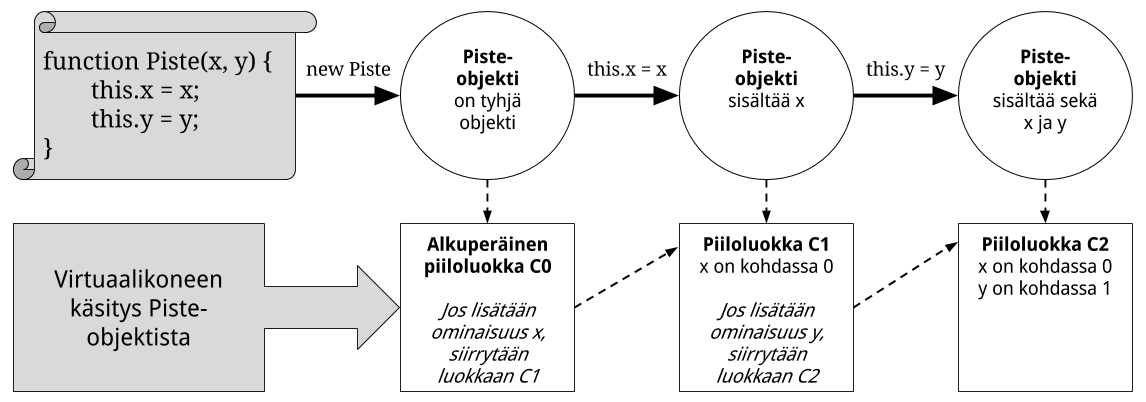
\includegraphics[width=\textwidth]{hidden-classes}
    \caption{Esimerkki piiloluokkien toimintaperiaatteesta}
     \centering
     \label{fig:hiddenclass}
\end{figure}

\subsection{Välimuistit}

(Inline cache)

\subsection{Roskienkeräys}

(Garbage collection)

\subsection{Staattinen kertasijoitusmuoto}

(Static single assignment form, SSA)
\section{Toteutusten vertailua}
\section{Tulevaisuus}

Brendan Eichin mukaan JavaScriptistä on tullut jo kliseenomaisesti ''Webin assemblykieli''~\cite{webassembly}. JavaScript-ohjelmia suoritetaan käytännössä jokaisella alustalla ja kehittäjät ovat alkaneet tehdä kääntäjiä, jotka kääntävät muita ohjelmointikieliä, vanhoja tai uusia, JavaScriptiksi. Tämä lisää painetta parantaa virtuaalikoneiden suorituskykyä ja lisätä matalamman tason rajapintoja kääntäjäohjelmoijien hyödynnettäväksi.

Asm.js~\cite{asmjs} on epävirallinen standardi JavaScriptin osajoukosta, jota on mahdollista kääntää tehokkaaksi konekoodiksi. Sen idea on olla toimivaa JavaScript-koodia, mutta mahdollistaa tehokas kääntäminen suoraan konekoodiksi. Se onnistuu kertomalla virtuaalikoneelle, että koodi on asm.js-muotoista ja tarjoamalla tyyppivihjeitä. Tässä esimerkki kokonaislukujen summafunktiosta asm.js-koodina:
\begin{lstlisting}
"use asm"; // Kerrotaan, että koodi on asm.js-muotoista.
function integerSum(x, y) {
  x = x|0; y = y|0;
  return (x + y)|0;
}
\end{lstlisting}
Esimerkissä kokonaislukuparametreista annetaan vihjeet tekemällä funktion alussa bittitason tai-operaatio: \texttt{x = x|0}. Jos \texttt{x}:n arvo ei ole kokonaisluku, esimerkiksi \texttt{undefined} tai jokin olio, operaatio muuttaa sen kokonaisluvuksi. Jos virtuaalikone tukee asm.js-kääntämistä, tyyppivihje kertoo virtuaalikoneelle, että parametri tulee aina olemaan kokonaisluku. Virheelliset tyypit voidaan huomata staattisilla työkaluilla suorittamatta koodia. JavaScriptin aritmetiikka toimii aina liukuluvuilla, joten sen takia myös summan tulos pitää muuttaa kokonaisluvuksi.

Mozillan OdinMonkey-kääntäjän lisäksi myös Googlen V8-virtuaalikoneen kehittäjät suunnittelevat tukea asm.js-optimoinneille TurboFan-kääntäjän avulla~\cite{turbofan}. Asm.js:n tueksi JavaScriptiin on tuotu lisää suorituskykyä parantavia toimintoja, kuten \textit{SIMD-käskyt}~\cite{webassembly}. SIMD tulee sanoista \textit{Single Instruction Multiple Data}, joka tarkoittaa suomeksi: ''Yksi käsky, useita data-alkioita''. SIMD-käskyjen avulla pystytään hyödyntämään prosessorien mahdollisuutta käsitellä useita data-alkioita, kuten vektoreita, yhdellä konekäskyllä. SIMD-käskyjen hyödyt tulevat esille, kun jokin keskeinen algoritmi täytyy saada mahdollisimman nopeaksi.

Yleensä JavaScript-ohjelmat käyttävät vain yhtä säiettä, joten ne eivät hyödynnä moniytimisiä prosessoreja kovin hyvin. Vaikka kielessä on jo Web Worker -rajapinta, joka mahdollistaa ohjelman jakamisen rinnakkaisiin tehtäviin. Niiden välinen kommunikaatio tapahtuu viestinvälityksellä, joka on melko hidasta. Tukea rinnakkaisohjelmoinnille halutaan parantaa tuomalla muun muassa \textit{SharedArrayBuffer}-rajapinta, eli jaettu taulukkopuskuri, ja atomiset operaatiot. Nämä yhdessä mahdollistavat matalan tason rinnakkaisohjelmoinnin, joka hyödyttää varsinkin raskasta laskentaa vaativia sovelluksia kuten pelejä.

Asm.js alkoi kokeellisena toteutuksena, mutta nyt selainvalmistajat ja standardoijat kehittävät yhdessä virallista Webin konekieltä, jota he kutsuvat nimellä WebAssembly~\cite{webassembly}. Sen on tarkoitus tarjota matalan tason binääriformaatti, jota kääntäjät voivat tuottaa. Koska WebAssembly on tiiviissä binäärimuodossa, sitä ei tarvitse purkaa, kuten pakattua JavaScript-koodia, eikä jäsentää uudelleen selaimessa. WebAssemblyn tavoite ei ole korvata JavaScript-koodia ja nykyistä kehitystapaa, vaan tarjota parempi tuki myös käännetyille ohjelmille, jotka aikaisemmin ovat toimineet helposti haavoittuvina selainlaajennuksina.

% TODO: SoundScript in V8, Transpilers!
\section{Yhteenveto}

JavaScript on löytänyt tiensä monille eri alustoille ja se on kasvattanut suosiotaan kehittäjien keskuudessa. Kukaan tuskin osasi ennustaa JavaScriptin tulevaisuutta, kun se luotiin. Se on käytännössä korvannut Javan ja muut laajennuksiin perustuvat kielet selaimista. Tämä ei olisi mahdollista ilman virtuaalikonekehittäjien panosta suorituskyvyn parantamiseksi.

Googlen innovatiivinen työ V8:n kanssa on kannustanut muita virtuaalikoneiden kehittäjiä parantamaan virtuaalikoneidensa suorituskykyä. Siirtyminen pelkästä tulkista useisiin JIT-kääntäjiin on parantanut suorituskykyä huomattavasti aikaisempaan arkkitehtuuriin verrattuna.

Tämänhetkisten optimointimenetelmien riippuvuus staattisesta käytöksestä vähentää niiden hyödyllisyyttä todellisissa sovelluksissa. Ainakin Google kertoo siirtävänsä huomionsa raa'asta suorituskyvystä yleisiin käyttötapauksiin ja sovelluskehyksiin. Onkin tärkeää opetella käyttämään työkaluja, joilla oman sovelluksen suorituskykyä voi mitata, sen sijaan, että opettelisi ulkoa optimointikikkoja. Virtuaalikoneet muuttuvat niin nopeaa tahtia, että se mikä vielä eilen oli hidasta voi olla huomenna jo nopeaa.

Virtuaalikoneiden kehittäjät julkaisevat jatkuvasti blogiviestejä uusista ominaisuuksista ja optimointimenetelmistä. Microsoft kertoi juuri avaavansa oman toteutuksensa avoimeksi lähdekoodiksi ja näin auttaa kaikkia toteutuksia jakamalla ideoitaan. JavaScriptin tulevaisuus vaikuttaa kirkkaalta ja Brendan Eichin, JavaScriptin luojan, sanoihin on hyvä päättää: ''Always bet on JS''~\cite{beton}.

%Vaikka JavaScriptin suunnittelijoilla ei voinut olla käsitystä mihin kaikkeen JavaScriptia tultaisiin käyttämään, he onnistuivat luomaan \textbf{hitin}. Alkuvaiheessa kukaan ei varmaankaan osannut ennustaa kielen tulevaa menestystä, eikä menestys olisi ollut mahdollinen ilman toteuttajien innovaatioita.

%Googlen innovatiivinen työ V8:n kanssa on kannustanut muita virtuaalikoneiden kehittäjiä parantamaan virtuaalikoneidensa suorituskykyä. Siirtyminen pelkästä tulkista eritasoisiin JIT-kääntäjiin on parantanut suorituskykyä huomattavasti aikaisempaan arkkitehtuuriin verrattuna.

%Nykyinen trendi käyttää JIT-kääntäjiä ja olettaa ohjelmien staattinen käyttäytyminen voi kuitenkin olla huono idea pidemmällä tähtäimellä. Vaikka virtuaalikoneet näyttävät nopeilta suorituskykytesteissä, voi verkkopalveluiden todelliset käyttäytymismallit olla dynaamisempia. Korkean tason ohjelmointikielen ohjelmoijan ei pitäisi tarvita tietää virtuaalikoneen sisäisestä toteutuksesta pystyäkseen kirjoittamaan tehokasta koodia.

%Virtuaalikoneiden kehittäjät tuntuvat jatkuvasti julkaisevan uusia viestejä blogeissaan, joissa he kertovat kuinka he ovat taas keksineet tai toteuttaneet uusia tapoja optimoida virtuaalikonettaan. Esimerkiksi V8:n kehittäjät kertovat blogissaan toteuttavansa uutta optimoivaa kääntäjää~\cite{turbofan}, joka pystyy optimoimaan enemmän erikoistapauksia kuin nykyinen ja mahdollistaa helpomman jatkokehityksen.

% V8 tiimi kertoo, että se on aikaisemmin keskittynyt vain raa'an suorituskyvyn parantamiseksi ja seuraava vaihe on keskittyä sovelluskehyksiin ja käytännön käyttötapauksiin!

% --- References ---

\bibliographystyle{babplain-lf}
%\bibliographystyle{babalpha-lf}
\pagebreak
\RaggedRight % Disable justifying, because it looks horrible with long links.
\bibliography{references}


% --- Appendices ---

% uncomment the following

% \newpage
% \appendix
% 
% \section{Esimerkkiliite}

\end{document}